\chapter{Музыкальные композиции}
\label{ch:musical-composition}
Глава посвящена исследованию музыкальных композиций. 
С помощью SPARQL-запросов, вычисляемых на объектах типа <<музыкальная композиция>> в~Викиданных, 
получены списки музыкальных композиций, список наиболее плодовитых композиторов, 
найдены популярные музыкальные жанры. 
Получен список музыкальных произведений в Викиданных, 
для которых будет законно зарузить их аудиозапись на Викисклад, поскольку истек срок копирайта.

\section{Число <<Музыкальных композиций>> и жанры}

\marginnote{Используемые в запросах объекты: <<\wdqName{музыкальное произведение/композиция}{105543609}>>;
используемое свойство: <<\wdProperty{31}{экземпляр}>>.}

Построим список всех музыкальных композиций с помощью запроса~\ref{lst:musical_composition}.

\begin{lstlisting}[ 
    language=SPARQL,
    caption={\href{https://w.wiki/9U7i}{Список всех  музыкальных композиций}\protect\footnotemark},
    label=lst:musical_composition,
    texcl,
    numbers=none
    ]
# List of all musical compositions
SELECT ?music ?musicLabel WHERE
{        # instance of musical work/composition
  ?music wdt:P31 wd:Q105543609. 
  SERVICE wikibase:label { bd:serviceParam wikibase:language "ru,en" }
}
\end{lstlisting}%
\footnotetext{Получено: \num{5495} записей на 2017 год и \num{150,5} тыс. записей на~2023 год. 
        Ссылка на~SPARQL-запрос: \href{https://w.wiki/9U7i}{https://w.wiki/9U7i}.}

Наиболее полными и проработанными примерами музыкальных композиций на Викиданных являются: <<\wdqName{Волшебная флейта}{5064}>>, <<\wdqName{К Элизе}{11980}>>, <<\wdqName{Реквием}{207875}>>, <<\wdqName{Маленькая ночная серенада}{12025}>>, <<\wdqName{Соната си синор}{63681379}>>.

В 2022 году по запросу~\ref{lst:musical_composition} найдено \num{106,7} тыс. музыкальных композиций, 
а~в~2023~--- \num{150,5} тыс., вместо \num{5,5} тыс. в~2017 году. 
Увеличение числа композиций связано с тем, что эти объекты Викиданных являются теперь не экземплярами объекта «музыкальное произведение», а экземплярами различных подклассов «музыкальное произведение». При поиске подклассов объекта «музыкальное произведение» можно найти такие жанры: <<\wdqName{песня}{7366}>>, <<\wdqName{духовная песня}{856713}>>, <<\wdqName{гимн}{484692}>>. Более подробно анализ музыкальных жанров будет представлен в разделе <<Количество музыкальных произведений по~жанрам>> на~с.~\pageref{chapter:Number-of-musical-works-by-genre}.

Диаграмма~\ref{fig:hier-music} показывает, как различные музыкальные классы связаны друг с другом и как они организованы в Викиданных. Это помогает пользователям лучше понять структуру и организацию информации о музыкальных классах в Викиданных.

\todoVlad{\TODO Владимир, так не годится писать плейнтекстом: <<на стр. 96>>, 
поскольку, например, в этом PDF-файле всего 49 страниц. 
Используйте команду pageref с аргументом label, 
который задаётся в~начале того раздела, на который Вы хотите сослаться. 
И между предлогом и словом нужен неразрывный пробел. 
Тогда получится, например так:} 
\begin{verbatim}
на~с.~\pageref{ch:BucketsAndBalls}. 
\end{verbatim}
\todoVladWithoutCounter{Здесь в начале метки ``ch:BucketsAndBalls'' стоит ``ch''~--- 
это сокращение от chapter (глава), 
чтобы не путать с другими метками (таблицами, рисунками).}
\answerVlad{Готово.}

\todoVlad{Добавьте текстовое описание к рис.~\ref{fig:hier-music}.\\  
P.S. Владимир, не удаляйте эти блоки с заданиями из текста. 
Так мне будет проще проверять}
\answerVlad{Готово.}

\answerVlad{Владимир, когда задание выполнено, 
то добавляйте такой зелёный блок текста, 
пишите в нём <<Готово>> или <<Сделано>>. 
Либо напишите пояснение, что не сделано и объясните~--- почему.}


\begin{marginfigure}[0\baselineskip]
	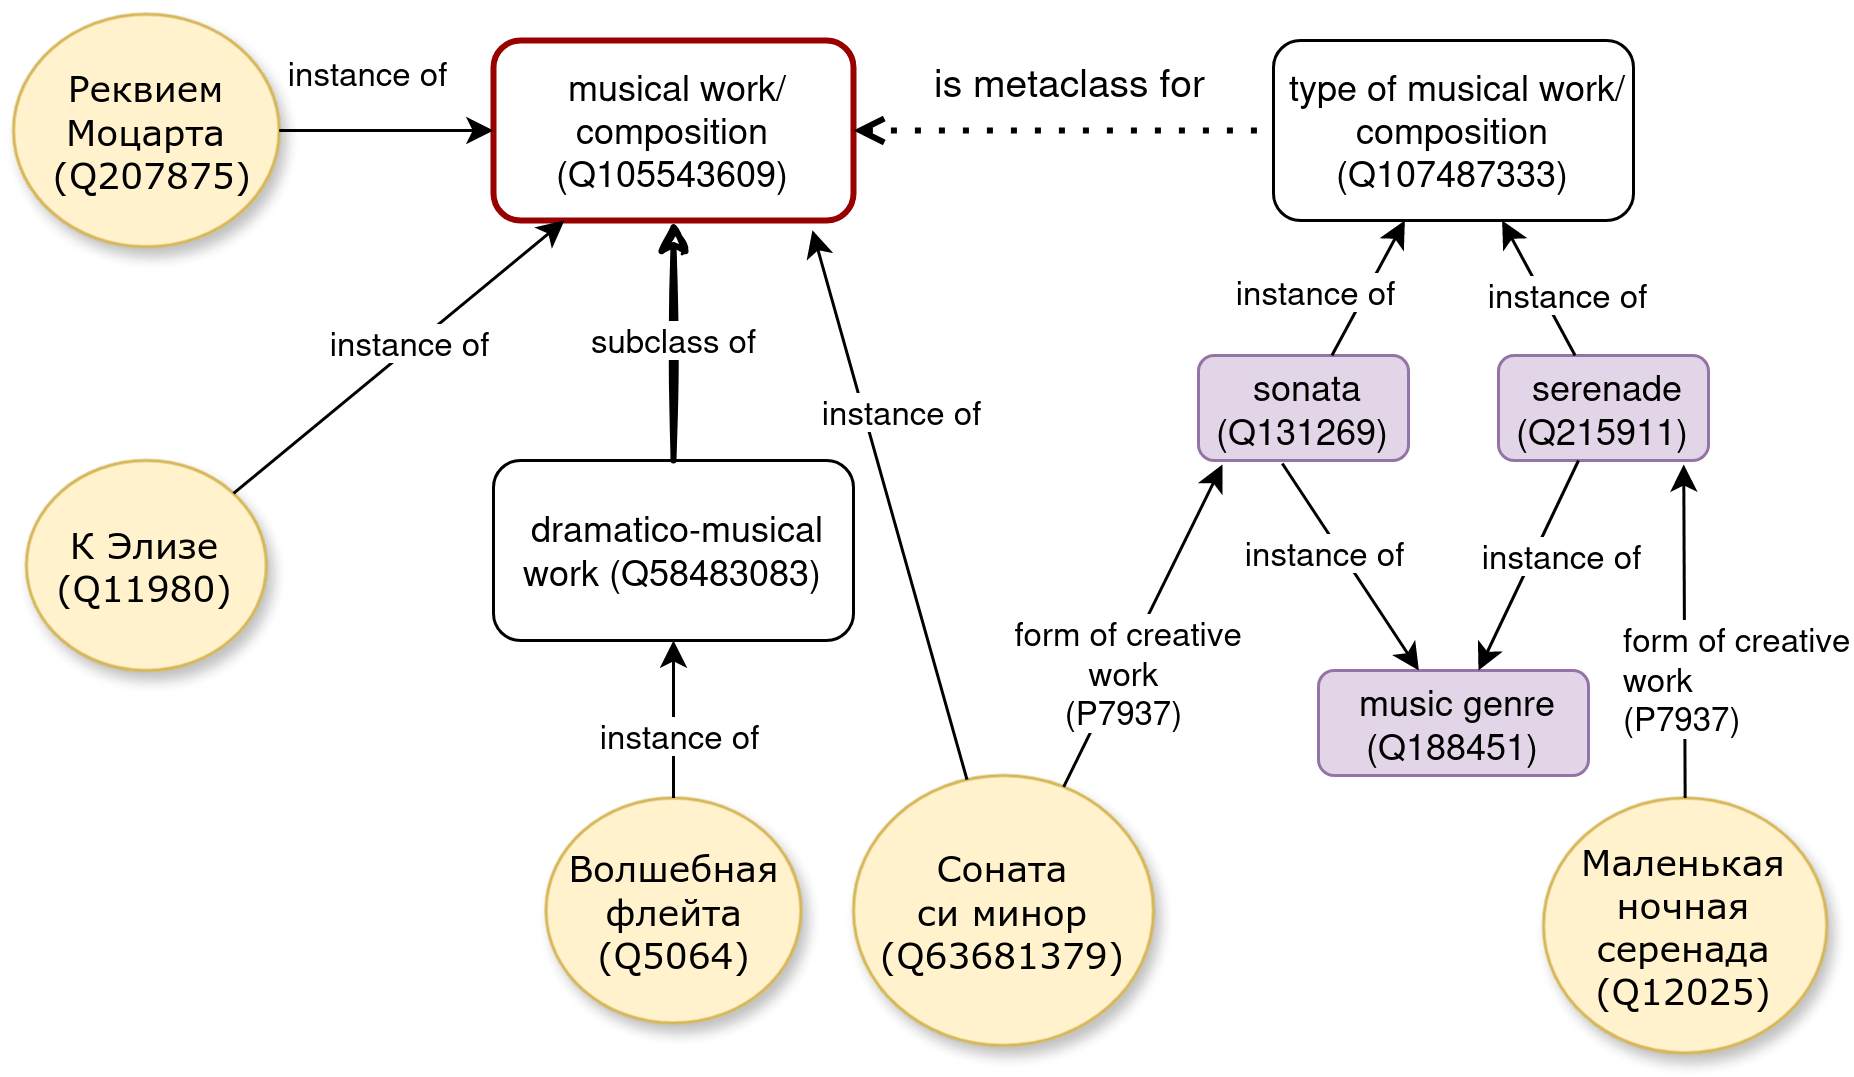
\includegraphics[width=1\textwidth]{./chapter/musical_composition/hierarchy_of_music_classes_WD_2023.png}
	\caption[Иерархия музыкальных классов]{Фрагмент иерархии музыкальных классов в Викиданных, 2023 год}%
	\label{fig:hier-music}%
\end{marginfigure}
Найдём количество музыкальных композиций в каждом жанре с помощью запроса~\ref{lst:music_in_each_subclass}.

\begin{lstlisting}[ 
    language=SPARQL,
    caption={\href{https://w.wiki/9U7w}
                  {Количество музыкальных композиций в каждом подклассе}\protect\footnotemark},
    label=lst:music_in_each_subclass,
    xleftmargin=18pt,
    numbers=left,
    ]
# Number of musical works in each subclass
SELECT ?type (COUNT(?music) AS ?count) ?typeLabel WHERE 
{                      # subclass of musical composition
                 ?type wdt:P279* wd:Q105543609.      
  ?music wdt:P31 ?type.
         # instance of this subclass
  SERVICE wikibase:label { bd:serviceParam wikibase:language "ru, en" }
}
GROUP BY ?type ?typeLabel
ORDER BY DESC (?count)
\end{lstlisting}%
\footnotetext{Получено: 9 подклассов музыкальных композиций на 2024 год. Ссылка на SPARQL-запрос: \href{https://w.wiki/9U7w}{https://w.wiki/9U7w}.}

\marginnote[6\baselineskip]{%
        \label{question:music_comp}
        \MarginQuestion
        В 9 подклассов <<\wdqName{musical work/composition}{105543609}>> , полученных в запросе~\ref{lst:music_in_each_subclass}, входят объекты <<\wdqName{incipit}{1161138}>> (<<начальные слова>>) и объект <<\wdqName{Маска}{1907293}>>, то есть это не~музыкальные вещи. Нужно добавить в запрос исключение этих двух объектов

        См. ответ~\ref{lst:music_in_each_subclas_2} на с.~\pageref{answer:music_in_each_subclas_filter}.
}

В этом запросе~\ref{lst:music_in_each_subclass} мы используем только левую часть рис.~\ref{fig:hier-music}, а именно объект  <<\wdqName{musical work/composition}{105543609}>>. Поэтому в подклассах нет ни сонаты, ни серенады.

Теперь напишем два запроса таким образом, чтобы запрос~\ref{lst:Number_of_types_of_musical_works_1} выявлял экземпляры объекта типа <<\wdqName{type of musical work/composition}{107487333}>>,а запрос~\ref{lst:Number_of_types_of_musical_works_2} экземпляры объекта <<\wdqName{music genre}{188451}>>. Эти запросы задействуют правую часть рис.~\ref{fig:hier-music}. В результате мы увидим такие жанры, как соната и серенада.

\begin{lstlisting}[ 
    language=SPARQL,
    caption={\href{https://w.wiki/9U8o}
                  {Экземпляры объекта <<\wdqName{type of musical work/composition}{107487333}>>}\protect\footnotemark},
    label=lst:Number_of_types_of_musical_works_1,
    texcl
    ]
# Number of types of musical works
SELECT ?type ?typeLabel WHERE 
{                # type of musical work
  ?type wdt:P31 wd:Q107487333.      
  SERVICE wikibase:label { bd:serviceParam wikibase:language "ru, en" }
}
\end{lstlisting}%
\footnotetext{Получено: 280 типов музыкальных работ на 2024 год. Ссылка на SPARQL-запрос: \href{https://w.wiki/9U8o}{https://w.wiki/9U8o}.}

\begin{lstlisting}[ 
    language=SPARQL,
    caption={\href{https://w.wiki/9UAP}
                  { Экземпляры объекта <<\wdqName{music genre}{188451}>>}\protect\footnotemark},
    label=lst:Number_of_types_of_musical_works_2,
    texcl
    ]
# Number of types of musical works
SELECT ?type ?typeLabel WHERE 
{                # type of musical work
  {?type wdt:P31 wd:Q188451} .
  SERVICE wikibase:label { bd:serviceParam wikibase:language "ru, en" }
}
}
\end{lstlisting}%
\footnotetext{Получено: 5809 музыкальных жанров на 2024 год. Ссылка на SPARQL-запрос: \href{https://w.wiki/9UAP}{https://w.wiki/9UAP}.}

Объединим типы музыкальных работ и музыкальные жанры, получаем запрос~\ref{lst:Number_of_genres_and_types_of_musical_works}.

\begin{lstlisting}[ 
    language=SPARQL,
    caption={\href{https://w.wiki/9UAX}
                  {Суммарное число музыкальных композиций в подклассах}\protect\footnotemark},
    label=lst:Number_of_genres_and_types_of_musical_works,
    xleftmargin=18pt,
    numbers=left,
    ]
# Number of genres and types of musical works
SELECT ?type ?typeLabel WHERE 
{                # type of musical work/composition
  {?type wdt:P31 wd:Q107487333} UNION 
  {?type wdt:P31 wd:Q188451} .
                 # music genre
  SERVICE wikibase:label { bd:serviceParam wikibase:language "ru, en" }
}
\end{lstlisting}%
\footnotetext{Получено:  6089 музыкальных типов и жанров на 2024 год. Ссылка на~SPARQL-запрос: \href{https://w.wiki/9UAX}{https://w.wiki/9UAX}.}

Мы ищем объекты, которые являются либо экземплярами <<\wdqName{type of musical work/composition}{107487333}>>, либо <<\wdqName{music genre}{188451}>>. В запросе~\ref{lst:Number_of_genres_and_types_of_musical_works} мы используем команду \lstinline|UNION| в~строке~4, чтобы объединить результаты поиска обоих типов объектов.

Допишем запрос~\ref{lst:Number_of_genres_and_types_of_musical_works}, чтобы он подсчитал число музыкальных произведений (без дубликатов), которые имеют такой музыкальный тип или жанр. Получим следующий запрос~\ref{lst:The_total_number_of_musical_works_for_subclasses}.
\begin{lstlisting}[ 
    language=SPARQL,
    caption={\href{https://w.wiki/9XWq}
                  {Суммарное число музыкальных композиций в подклассах}\protect\footnotemark},
    label=lst:The_total_number_of_musical_works_for_subclasses,
    texcl
    ]
SELECT (SUM(?numberOfmusic) AS ?totalNumberOfmusic) WHERE {
  {
    SELECT (COUNT(DISTINCT ?music) AS ?numberOfmusic) WHERE {
      {?music wdt:P31 wd:Q107487333} UNION {?music wdt:P31 wd:Q188451}.
      {?music wdt:P279 ?type}.
      SERVICE wikibase:label { bd:serviceParam wikibase:language "ru, en" }
    }
    GROUP BY ?type ?typeLabel
  }
}
\end{lstlisting}%
\footnotetext{Получено: 8327 музыкальных произведений на 2024 год. Ссылка на~SPARQL-запрос: \href{https://w.wiki/9XWq}{https://w.wiki/9XWq}.}

\todoVlad{
\emph{Задача с исключением~--- на поля и в <<Ответы>>.}\\
В 9 подклассов ``musical work/composition'', 
полученных в запросе~\ref{lst:music_in_each_subclass},
входят объекты ``incipit (Q1161138)'' (<<начальные слова>>) 
и объект Маска (wd:Q1907293), то есть это не~музыкальные вещи. 
Нужно добавить в запрос исключение этих двух объектов, 
вижу два варианта: или функция FILTER (неравенство) или MINUS. 
Примеры скриптов с~MINUS 
посмотрите на странице ВВ \href{https://ru.wikiversity.org/?curid=23632}
                               {Программирование Викиданных/Страны}. 
Отмечу, что в результатах есть ещё <<маска>> с маленькой буквы~--- 
это музыкальный жанр, его не нужно исключать.  
\\
На полях напишите это задание (исключение). 
В раздел <<Ответы>> добавьте свой вариант с решением.}
\answerVlad{Готово.}

\todoVlad{
\emph{Добавление.}\\
После запроса~\ref{lst:music_in_each_subclass} 
обратите внимание читателя, 
что в этом запросе используется только левая часть рис.~\ref{fig:hier-music}, 
а именно:  ``musical work/composition (Q105543609)''. 
Поэтому в~подклассах нет ни сонаты, ни серенады. 

Теперь напишем запрос, в котором будут искаться экземпляры объектов 
``type of musical work/composition (Q107487333)'' и ``music genre (Q188451)''.
В результатах тогда появятся жанры: соната и серенада.

\vspace{12pt}
Предлагаю такой запрос \url{https://w.wiki/9U8o}, 
в этом запросе ищутся экземпляры ``type of musical work (Q107487333)'',  
получаем 280 типов муз. работ. 

\vspace{12pt}
С помощью запроса \url{https://w.wiki/9UAP} получаем 5800 музыкальных жанров, 
это экземпляры объекта ``music genre (Q188451)''.

\vspace{12pt}
Объединим типы музыкальных работ и музыкальные жанры, получаем запрос: \url{https://w.wiki/9UAX}, 
получаем 6083 музыкальных типов и жанров. Приведите с пояснениями листинг этого запроса в тексте. 
Теперь Ваша задача, Владимир, дописать этот запрос, чтобы он подсчитал число 
музыкальных произведений (без дубликатов), которые имеют такой музыкальный тип или жанр. 
}
\answerVlad{Готово.}


\todoVlad{Общее пожелание. Добавьте к запросам, которые возвращают числа~--- данные за 2024 год, 
при этом оставляйте данные (число результатов) за предыдущие годы.}

Теперь подсчитаем общее суммарное число музыкальных произведений с учётом музыкальных композиций в подклассах. Для этого добавим в~запрос~\ref{lst:music_in_each_subclass} команду \lstinline|SUM()| в~строку~2 и удалим лишние строки, чтобы получить запрос~\ref{lst:The_total_number_of_musical_works_for_all_subclasses}.


\begin{lstlisting}[ 
    language=SPARQL,
    caption={\href{https://w.wiki/9Tc3}
                  {Суммарное число музыкальных произведений 
                   с~учётом музыкальных композиций в~подклассах}\protect\footnotemark},
    label=lst:The_total_number_of_musical_works_for_all_subclasses,
    xleftmargin=18pt,
    numbers=left,
    ]
# The total number of musical works for all subclasses 
SELECT (SUM(?count) AS ?sum) WHERE{
  SELECT (COUNT(?music) AS ?count) WHERE {
                         # subclass of musical work/composition
                   ?type wdt:P279* wd:Q105543609.
    ?music wdt:P31 ?type
  }        # instance of this subclass
}
\end{lstlisting}%
\footnotetext{Получено: 145~тыс. музыкальных произведений на 2022 год, 
    164~тыс. на 2023 год и 170~тыс. на 2024 год. 
    Ссылка на~SPARQL-запрос: \href{https://w.wiki/9Tc3}
                                  {https://w.wiki/9Tc3}.}

Можно записать этот код ещё короче. 
Переменная \lstinline|?type| нам не нужна, 
поэтому заменим её на \emph{безымянную переменную}, \index{SPARQL![]!безымянная переменная}
а~строки 5 и 6 поменяем местами, 
получаем запрос~\ref{lst:The_total_number_of_musical_works_for_all_subclasses_up}.

\begin{lstlisting}[ 
    language=SPARQL,
    caption={\href{https://w.wiki/9Td7}
                  {Суммарное число музыкальных произведений с~учётом музыкальных композиций 
                  в~подклассах (безымянная переменная)}\protect\footnotemark},
    label=lst:The_total_number_of_musical_works_for_all_subclasses_up,
    texcl,
    numbers=none
    ]
# Total number of musical works for all subclasses
SELECT (SUM(?count) AS ?sum) WHERE{
  SELECT (COUNT(?music) AS ?count) WHERE {
    ?music wdt:P31   # instance of
          [wdt:P279* wd:Q105543609].
  }        # subclass of musical work/composition
}
\end{lstlisting}%
\footnotetext{Идентичный запрос предыдущем, то же число результатов. Ссылка на~SPARQL-запрос: \href{https://w.wiki/9Td7}{https://w.wiki/9Td7}.}

По сравнению с 2017 годом, когда было получено \num{5494} записи, число записей увеличилось в десятки раз. Это связано с тем, что за 6 лет было добавлено множество новых музыкальных произведений, а также старых, которые не были учтены ранее.
Напишем скрипт~\ref{lst:Musical_comp_2018--2024} и посмотрим сколько новых и старых (то есть созданных до 2018 года) музыкальных произведений было добавлено в~Викиданные за~период с~2018 года по~2024 год.

\todoVlad{Здесь аналогично~--- замените, пожалуйста, 
2023 на 2024 и обновите результаты. 
Выше напишите <<за 6 лет>>, а не за пять лет.}
\answerVlad{Готово.}

\begin{lstlisting}[ 
    language=SPARQL,
    caption={\href{https://w.wiki/9aHW}{ Количество музыкальных композиций в период 2018--2024 годы}\protect\footnotemark},
    label=lst:Musical_comp_2018--2024,
    xleftmargin=18pt,
    numbers=left,
    ]
# The total number of musical works for all subclasses 
SELECT (SUM(?count) AS ?sum) WHERE{
  SELECT (COUNT(?music) AS ?count) WHERE{
    ?music wdt:P31 wd:Q105543609;  # is musical work/composition
           wdt:P577 ?date.         # has a publication date
    BIND(YEAR(?date) AS ?year)
   FILTER(?year > 2018)
  }
}
\end{lstlisting}%
\footnotetext{Получено: \num{4183} музыкальных произведений за 2018--2024 годы. Ссылка на SPARQ-запрос: \href{https://w.wiki/9aHW}{https://w.wiki/9aHW}.}

При использовании фильтрации\lstinline|FILTER| в запросе~\ref{lst:Musical_comp_2018--2024}, можно использовать такую тяжёлую конструкцию:

\text{\lstinline|FILTER(?date > "2018-01-01T00:00:00Z"^^xsd:dateTime)|} в строке 7.
В этом случае не требуется строка 6 с командой \lstinline|BIND|, что может упростить код.

В альтернативном (нашем) варианте мы получаем более читаемый код с использованием команды \lstinline|BIND| в строке 6 и переменной \lstinline|?year| в строке 7.

\todoVlad{Владимир, я вернул в запрос~\ref{lst:Musical_comp_2018--2024} нумерацию строк. 
Не понял, почему Вы удалили нумерацию. 
Можете посмотреть сканы в ТГ от 13 декабря, которые я Вам присылал, насчитал там 6 скриптов с нумерацией. 
Прошу вернуть нумерацию строк в те скрипты, на номера строк которых есть отсылки из текста.}
\answerVlad{Готово.}
\todoVlad{Владимир, в запросе~\ref{lst:Musical_comp_2018--2024} 
есть такая строка \lstinline|BIND(YEAR(?date) AS ?year)|. 
Забавно, но переменная ?year, задаваемая в этой строке, в скрипте не используется. 
Перепишите строку 7 с командой FILTER, чтобы использовалась переменная ?year. 
В тексте после запроса напишите, что\newline 
(1: вариант с FILTER) можно использовать такую тяжёлую конструкцию 
\lstinline|FILTER(?date > "2018-01-01T00:00:00Z"^^xsd:dateTime)|, 
но зато не нужна строка 6 с командой \lstinline|BIND|,\newline 
либо\newline
(2: вариант без FILTER) более читаемый код с командой \lstinline|BIND| 
и переменной \lstinline|?year|. \newline
В листинге будет только вариант (2), в тексте~--- оба. 
В тексте пишите строчки кода или команды SPARQL с помощью конструкции lstinline.}
\answerVlad{Готово.}


Запрос~\ref{lst:The_total_number_of_musical_works_for_all_subclasses_up} 
возвращает 170 тыс. музыкальных произведений, которые могут иметь или не~иметь дату публикации. 
В~запросе~\ref{lst:Musical_comp_2018--2024} в~строке~5 
мы требуем обязательного наличия свойства <<\wdProperty{577}{дата публикации}>> у музыкального произведения.
Таких произведений с заполненной датой публикации 
(и выключенной, 
 то есть закомментированной строкой~7 в~запросе~\ref{lst:Musical_comp_2018--2024}) найдено 55 тыс., 
то есть примерно в~3~раза меньше. 
Если фильтрация в~строке~7 запроса~\ref{lst:Musical_comp_2018--2024} включена, 
то получаем 4.2 тыс. новых произведений, опубликованных не~ранее 2018 года. 
Получается, что таких достоверно <<новых>> музыкальных произведений 
около 2\,\% (4.2 тыс.) от всех музыкальных произведений в Викиданных (170 тыс.).



\newpage
\section{Количество музыкальных произведений по годам}

Подсчитаем количество музыкальных произведений 
со второй половины XIX века до настоящего времени 
с~помощью запроса~\ref{lst:The_number_of_musical_compositions_for_every_10_years}. 
Этот запрос строит рис.~\ref{fig:diagram_10_years}, где 
указано число созданных произведений по десятилетиям. 


\index{SPARQL!wikibase!isSomeValue}
\begin{lstlisting}[ 
    language=SPARQL,
    caption={\href{https://w.wiki/9aHU}
                  {Количество музыкальных произведений, создаваемых каждое десятилетие}\protect\footnotemark},
    label=lst:The_number_of_musical_compositions_for_every_10_years,
    texcl,
    numbers=none
    ]
# The number of musical compositions for every 10 years
#defaultView:BarChart
SELECT (STR(?date) AS ?date_str) (COUNT(?composition) AS ?count) WHERE {
  ?composition wdt:P31 wd:Q105543609;     # instance of compostion
    wdt:P86 ?composer;                    # composition has a composer
    wdt:P577 ?publication.                # composition has a publication date
  BIND(YEAR(?publication) AS ?date)
  BIND((FLOOR(?date / 10 )) * 10  AS ?year)
  FILTER(?year > 1850)
  FILTER(?year < 2030) 
  FILTER (!wikibase:isSomeValue(?publication)) # field "date" must be filled
}
GROUP BY ?date
ORDER BY (?date)
\end{lstlisting}%
\footnotetext{Ссылка на SPARQL-запрос: \href{https://w.wiki/9aHU}{https://w.wiki/9aHU}.}


\newpage
\begin{marginfigure}[-5\baselineskip]
    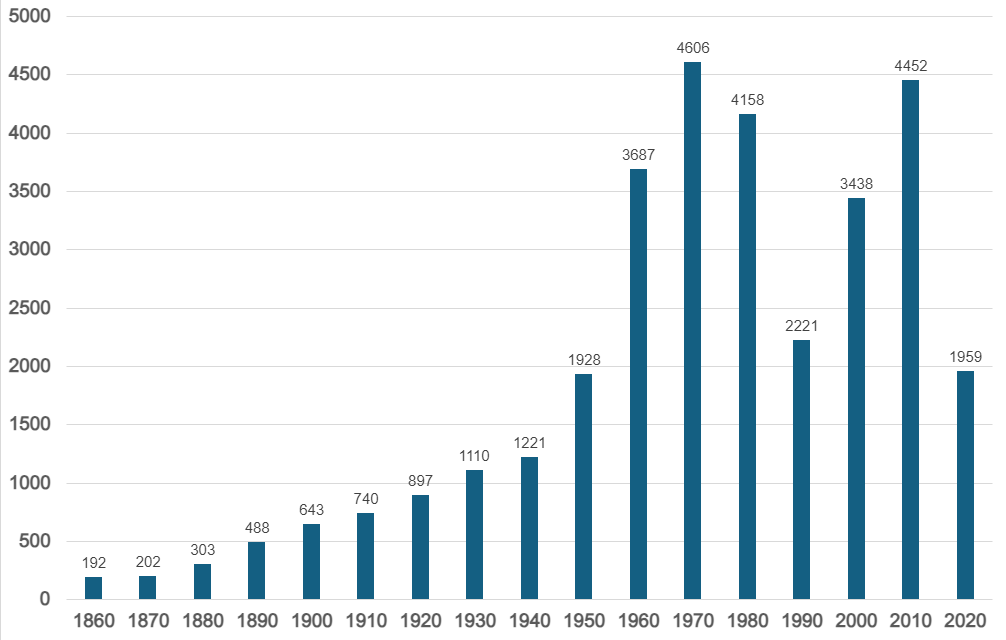
\includegraphics[width=1\textwidth]{./chapter/musical_composition/BarChart_of_The_number_of_music_compositions_for_every_10_years.svg.png}a
    \vspace{-7pt}
	\caption{Гистограмма количества музыкальных произведений, 
             создаваемых каждое десятилетие во всём мире со второй половины XIX века до настоящего времени}%
	\label{fig:diagram_10_years}%
\end{marginfigure}
%
Рис.~\ref{fig:diagram_10_years} показывает, что до 1890 года (1850--1890 годы) 
количество написанных музыкальных произведений невелико. 
После 1890 года (1890--1970 годы) начинается резкий подъём числа новых произведений 
и продолжается до нашего времени. 
Такое увеличение музыкальных произведений можно объяснить тем, 
что со временем появляются новые жанры и новые устройства для записи. 
На гистограмме (рис.~\ref{fig:diagram_10_years}) видим два пика: 1960--1990-е, 2000-е и 2020-е.

\todoVlad{Владимир, у скриншота (рис.~\ref{fig:diagram_10_years}) низкое качество 
(то есть текст размытый при увеличении), 
переснимите, пожалуйста, с большим разрешением. 
На рис.~\ref{fig:diagram_10_years} нужно сделать крупные подписи по обеим осям (название оси и числа). 
Можете доработать в графическом редакторе. 
Не забудьте новые версии рисунков загружать на Викисклад 
(можно поверх старых, чтобы не писать заново описание файла) 
и новые рисунки включайте в свою страницу в Викиверситете, то есть сюда: 
\textit{Программирование Викиданных/Музыкальные композиции}.}
\answerVlad{Готово.}


\section{Количество музыкальных произведений по десятилетиям в России}

Добавим в запрос~\ref{lst:music_in_genres_after2020} страну происхождения (<<Россия>> и <<СССР>>) 
музыкальных произведений, а~ограничение по годам в строках 7 и 8 уберём. 
Получим запрос~\ref{lst:The_number_of_musical_compositions_in_Russia_for_every_10_years}, 
подсчитывающий сколько отечественных музыкальных произведений было написано 
в каждом десятилетии с середины XIX века до настоящего времени.

\begin{lstlisting}[ 
    language=SPARQL,
    caption={\href{https://w.wiki/9UR2}
                  {Количество музыкальных произведений в Росии и СССР 
                   за каждые 10 лет}\protect\footnotemark},
    label=lst:The_number_of_musical_compositions_in_Russia_for_every_10_years,
    texcl 
    ]
# Number of musical compositions in Russia every 10 years
#defaultView:BarChart
SELECT (STR(?year10) AS ?date_str) (COUNT(?music) AS ?count) WHERE {
        {?music wdt:P17 wd:Q15180}    # country = USSR
  UNION {?music wdt:P17 wd:Q159}      # country = Russia
  UNION {?music wdt:P495 wd:Q159}     # country of origin = Russia
  UNION {?music wdt:P495 wd:Q15180}.  # country of origin =  USSR
  ?music wdt:P31 wd:Q105543609;  # is musical work/composition
         wdt:P86 ?composer;      # written by composer
         wdt:P577 ?date.         # has publication date

  FILTER (!wikibase:isSomeValue(?date)) # field "date" must be filled
  BIND(YEAR(?date) AS ?year)
  BIND((FLOOR(?year / 10 )) * 10  AS ?year10)
}
GROUP BY ?year10
ORDER BY ?year10
\end{lstlisting}%
\footnotetext{Ссылка на SPARQL-запрос: \href{https://w.wiki/9UR2}{https://w.wiki/9UR2}.}


\todoVlad{В скрипте выше также используйте предложения из замечания (4: Добавление). 
Надеюсь, тогда в следующем абзаце не придётся писать, что 
<<количество музыкальных произведений в России и СССР очень мало>>, 
поскольку это, конечно, не так.}
\answerVlad{При исправлении скрипта, он выдает 0 результатов \href{https://w.wiki/9f8B}{https://w.wiki/9f8B}.}

\newpage

\begin{marginfigure}[0\baselineskip]
	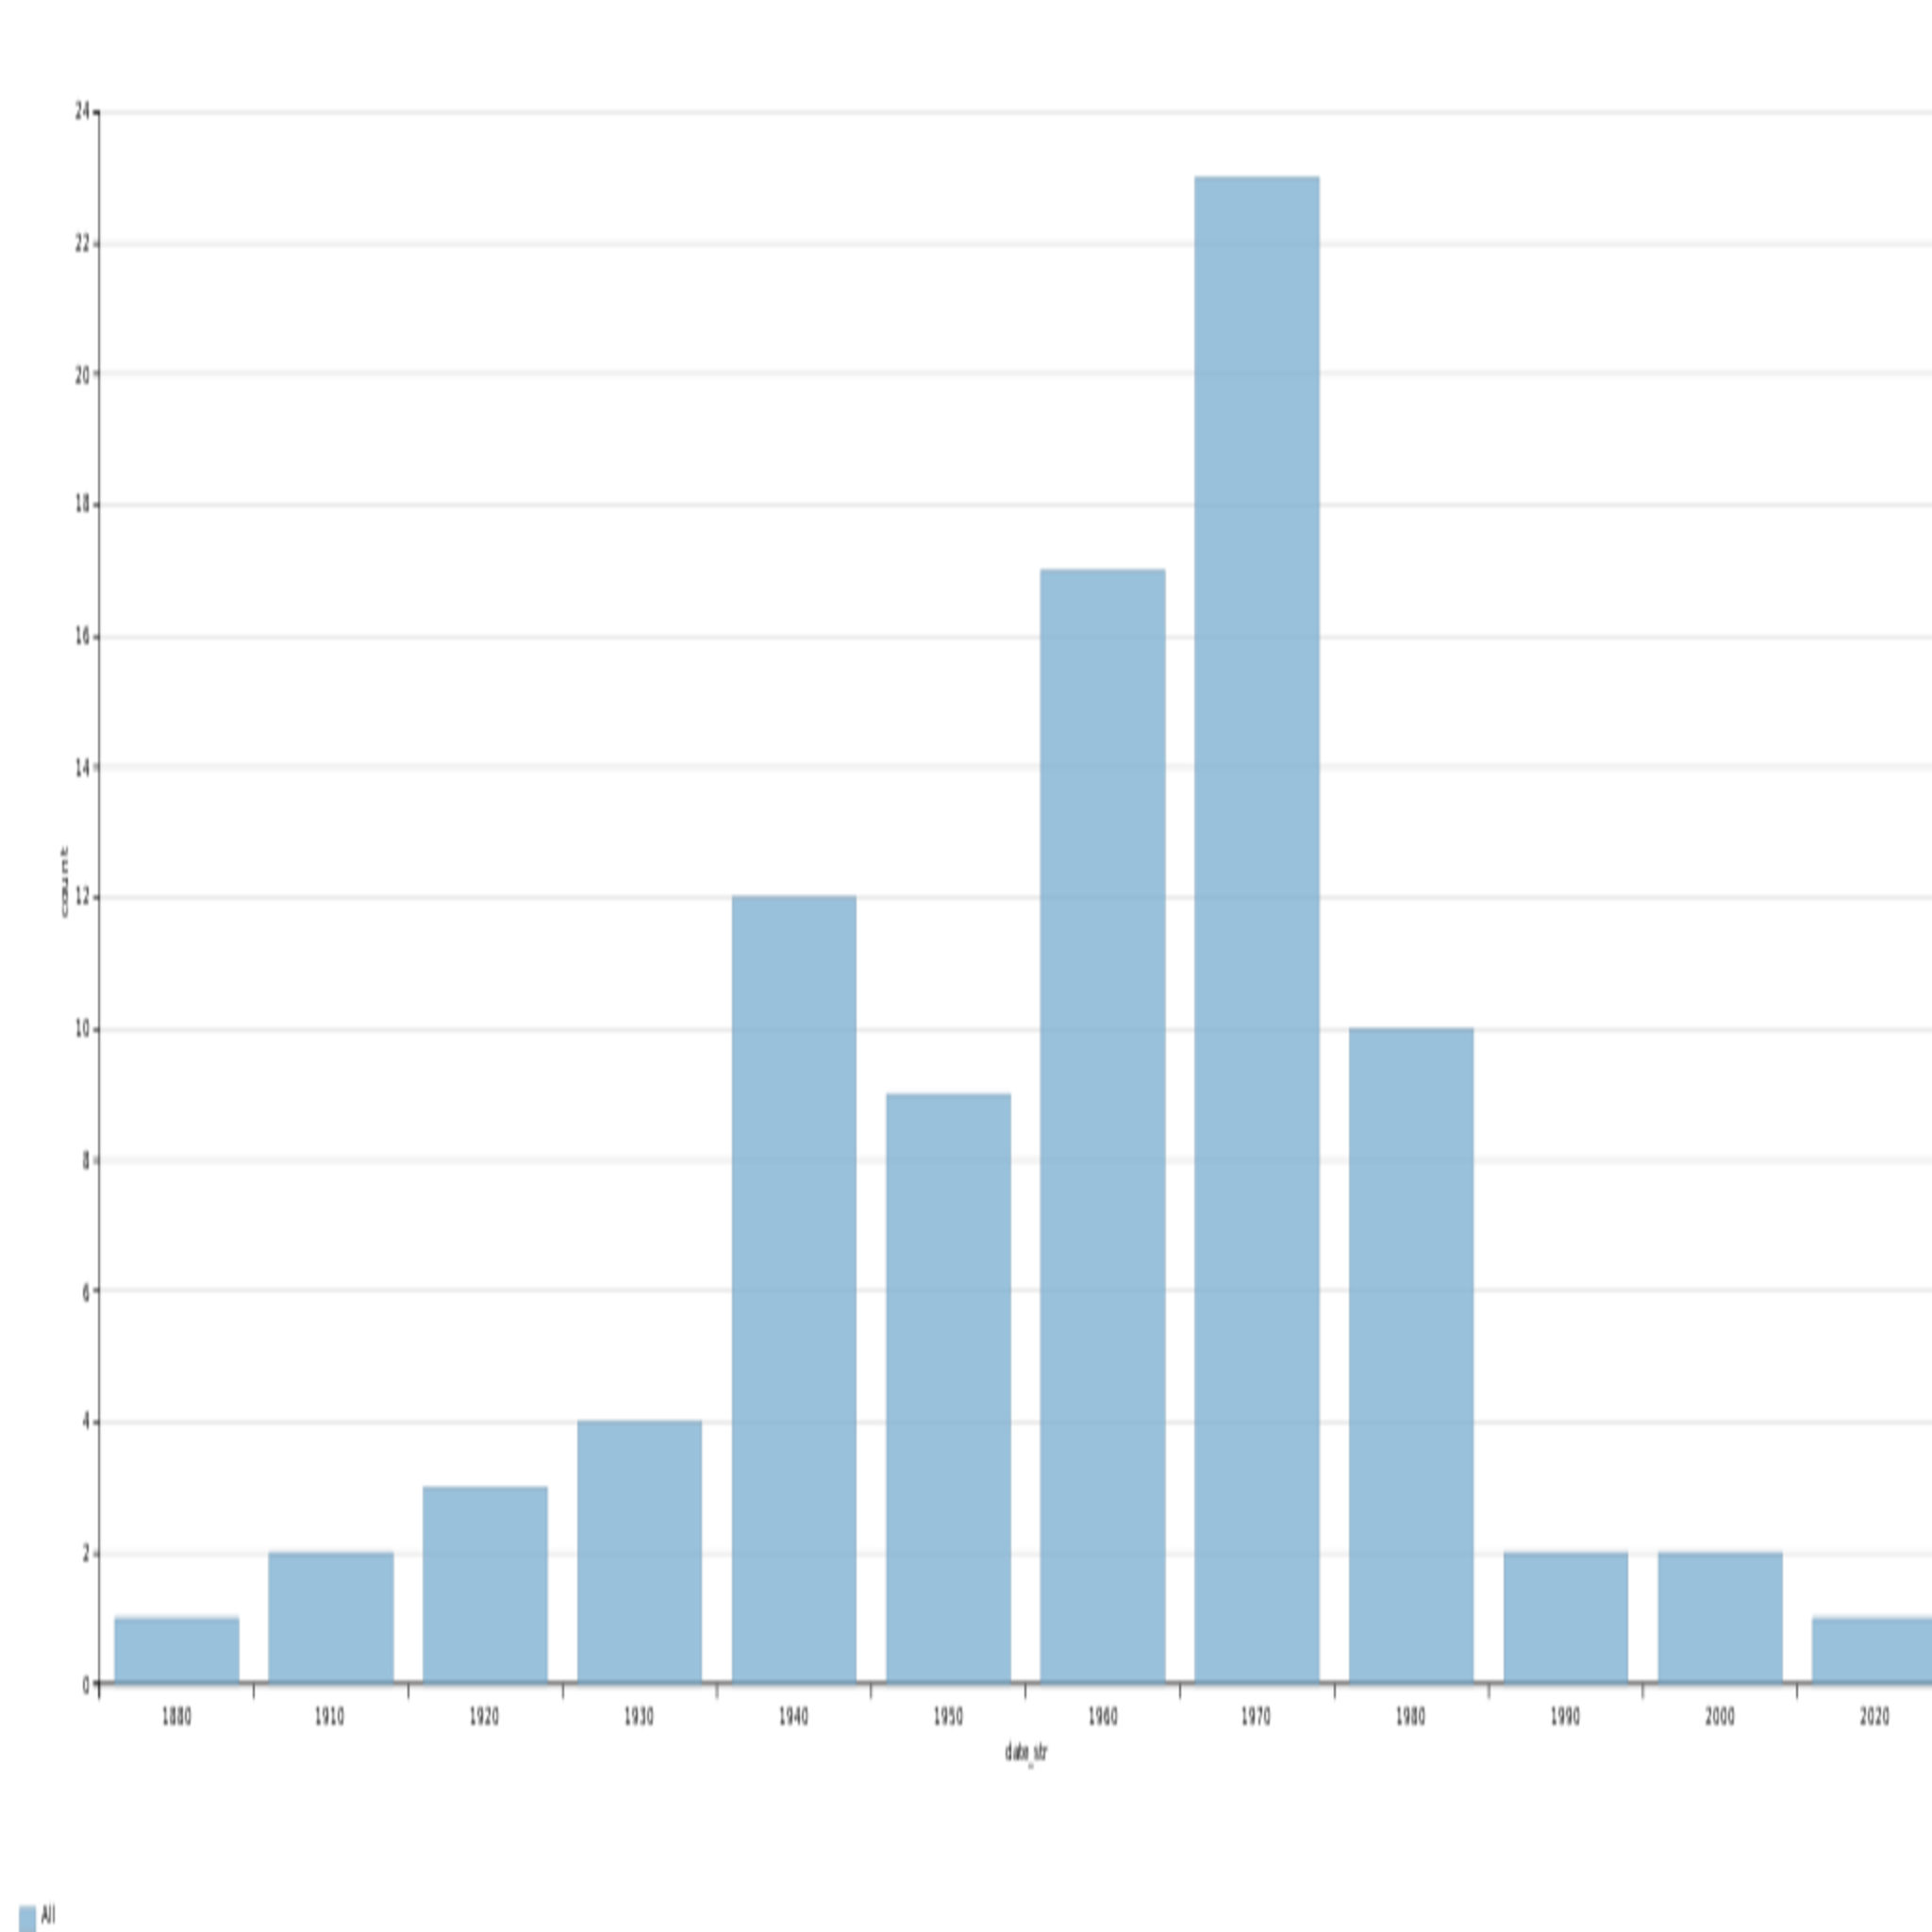
\includegraphics[width=1\textwidth]{./chapter/musical_composition/Barchart_of_The_number_of_music_compositions_in_Russia_and_USSR_every_10_years.svg.png}
    \vspace{-7pt}
	\caption{Гистограмма количества музыкальных произведений, 
             создаваемых каждое десятилетие в России и СССР с~XIX века до~настоящего времени}%
	\label{fig:diagram_10_yearsRussia}%

\end{marginfigure}

Количество музыкальных произведений в России и СССР очень мало (97). 
Проанализировав несколько песен, написанных в России, таких как: 
<<\wdqName{Песня без слов (Кино)}{101001315}>>, 
<<\wdqName{Музыка нас связала}{105724079}>>, 
<<\wdqName{Розовое вино}{57744615}>>, 
не~попавших в данный скрипт, стало понятно, 
что у~этих произведений отсутствует свойство <<\wdProperty{495}{Cтрана происхождения}>>.

Строка~9 запроса~\ref{lst:The_number_of_musical_compositions_in_Russia_for_every_10_years}~---  
\lstinline|wdt:P86 ?composer;|~--- 
требует наличия композитора у музыкального произведения. 
Если убрать эту строку (модифицированный запрос \href{https://w.wiki/9Ud9}
                                                     {https://w.wiki/9Ud9}), 
то получим произведения как с~композиторами, так и~без~них. 

Сравним результаты обоих скриптов на рис.~\ref{fig:chart}. 
Эта диаграмма показывает, что модифицированный запрос 
в основном выдаёт больше или столько же результатов, 
как и~исходный запрос~\ref{lst:The_number_of_musical_compositions_in_Russia_for_every_10_years}, 
что логично, потому что модифицированный запрос не имеет обязательного условия наличия композитора. 

Но есть исключения, например: 1880-е, 1960-е. 
Посмотрим список музыкальных композиции с~помощью запроса \href{https://w.wiki/9UdP}
                                                               {https://w.wiki/9UdP}. 
За 1880 год этот запрос выдает 5~результатов: 
<<\wdqName{Всенощное бдение}{16002554}>> (1 раз), 
\wdqName{String Quartet on the Theme B-la-F}{18660379} (4 раза). 
Вторая композиция повторяется 4 раза, поскольку в этом музыкальном объекте указаны 4~композитора. 

\marginnote[6\baselineskip]{%
        \label{question:music_unique}
        \MarginQuestion
       Как избавится от дубликатов в запросе~\ref{lst:The_number_of_musical_compositions_in_Russia_for_every_10_years}, то есть чтобы независимо от числа композиторов, музыкальные произведения не повторялись. 
        См. ответ~\ref{lst:Number_of_unique_musical_compositions} на с.~\pageref{answer:music_unique_answ}.
}

\todoVlad{Рядом с фразой указаны <<4~композитора>> поставьте на поля вопрос о том, 
как избавиться от дубликатов, то есть чтобы независимо от числа композиторов, 
музыкальные композиции не повторялись в списке результатов. 
Добавьте ответ в раздел <<Ответы>>, вот запрос для ответа с ключевым словом \lstinline|DISTINCT|: 
\href{https://w.wiki/9Udc}{https://w.wiki/9Udc}.
}
\answerVlad{Готово.}

\todoVlad{Со страницы 
Обсуждение:Программирование Викиданных/Музыкальные композиции 
взял следующую задачу, которую мы обсуждали. 
Сейчас есть две гистограммы: 
количество музыкальных произведений по всему миру (рис.~\ref{fig:diagram_10_years}) 
и по России (рис.~\ref{fig:diagram_10_yearsRussia}). 
Нужен третий рисунок: 
объедините данные этих двух рисунков и сделайте, например, в Excel'е так,  
чтобы за каждое десятилетие было два столбца (синий — весь мир, красный — Россия), 
см. как у Вас хорошо получилось на рис.~\ref{fig:chart}.\\
Также как на рис.~\ref{fig:chart}~--- подпишите над столбиками числа. 
}

\newpage
\todoVlad{Владимир, есть два раздела (выше):\\
(1) Количество музыкальных произведений по годам и\\ 
(2) Число композиций по десятилетиям в России.\\ 
У меня несколько вопросов и пожеланий, которые, надеюсь, Вы учтёте:\\

(A) Почему эти два раздела идут не подряд друг за другом, а разделены подразделом 
<<Количество музыкальных произведений по жанрам>>? 
Полагаю, что нужно переупорядочить разделы.\\

(Б) Почему так сильно различаются названия этих двух разделов (1) и (2)? 
Они же об одном и том же, только в первом музыка по десятилетиям во всём мире, 
а во втором --- только в России. Передумайте названия, чтобы они были более складными 
и гармоничными друг с другом. 
}

\begin{marginfigure}[0\baselineskip]
	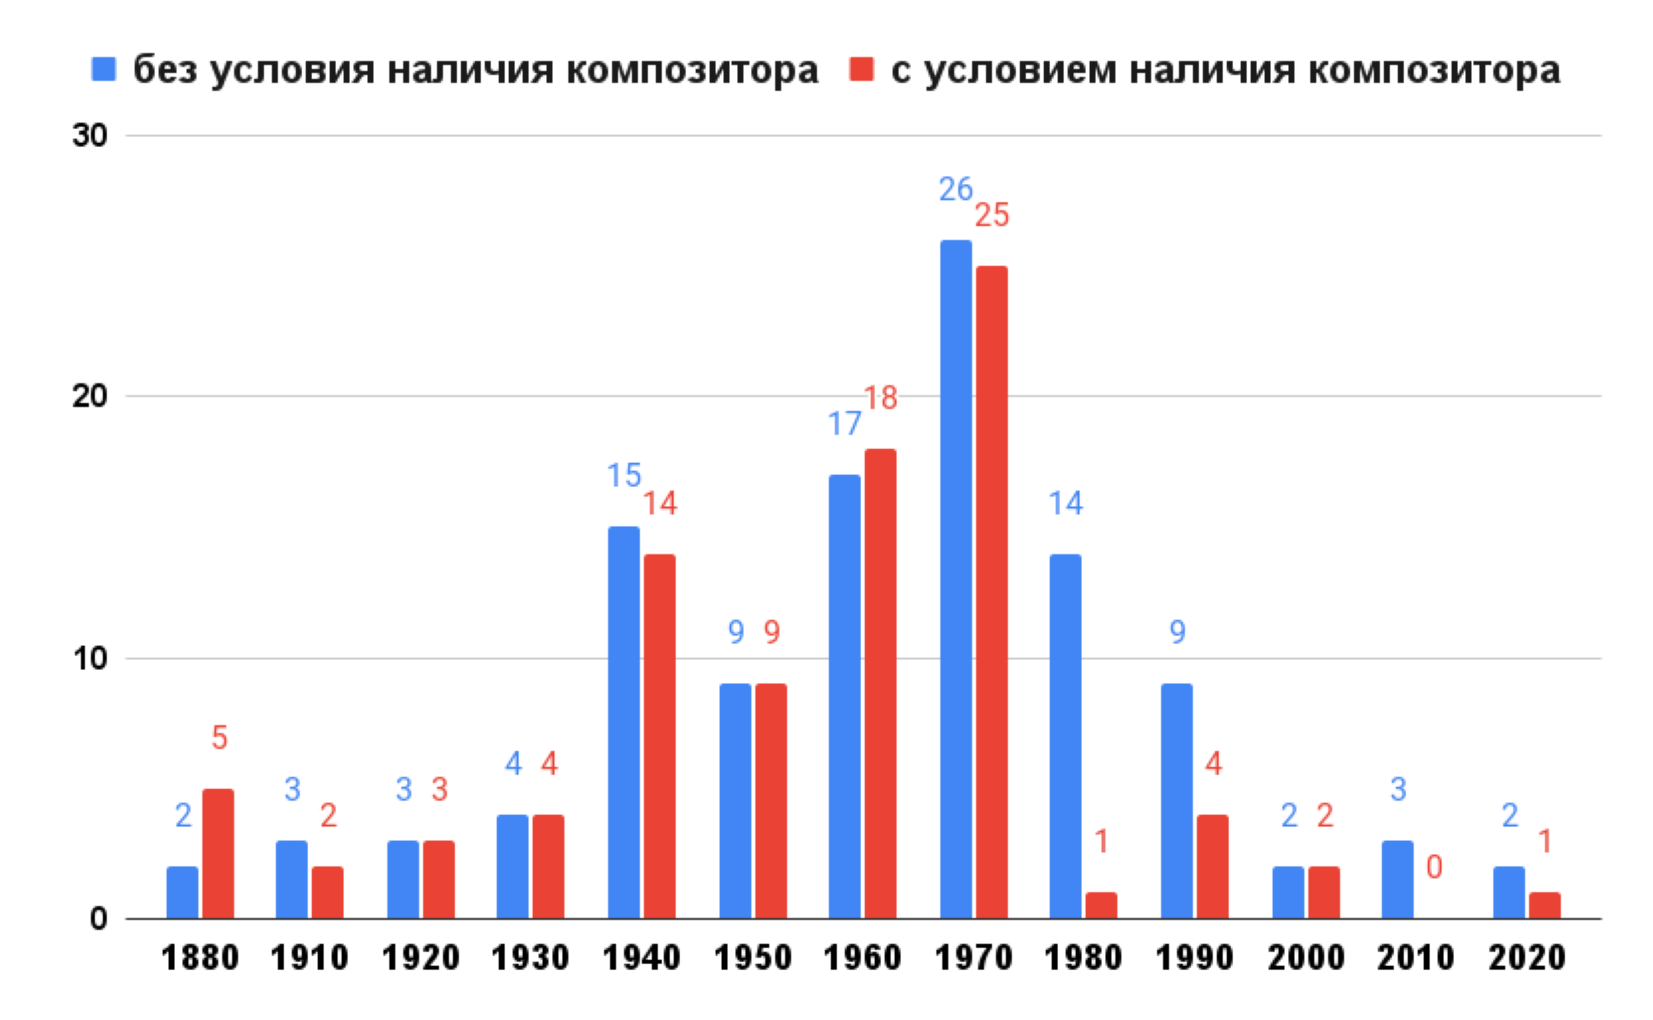
\includegraphics[width=1\textwidth]{./chapter/musical_composition/graph_of_comparison_of_readings.png}
	\caption{Сравнение числа музыкальных композиций по десятилетиям в России с условием наличия композитора и без него.}%
	\label{fig:chart}%
\end{marginfigure}

\todoVlad{По рис.~\ref{fig:chart}:\\
1) В легенде рисунка (т.е. у синего и красного квадратиков) 
вместо <<без условия наличия композитора>> напишите <<без композитора>>, 
вместо <<с условием наличия композитора>> напишите <<с композитором>>.\\
2) Подрисуночная подпись. Такая не годится, поскольку сейчас она не говорит о том, 
что именно на ней изображено, а говорит о том, что это результаты какого-то запроса.}
\answerVlad{Готово.}


\newpage
\section{Количество музыкальных произведений по жанрам}
\label{chapter:Number-of-musical-works-by-genre}

Найдём, в каких жанрах были написаны музыкальные произведения 
в пиках графика (рис.~\ref{fig:diagram_10_years}) 
и~изобразим жанры на~круговой диаграмме (рис.~\ref{fig:Genre_Chart_1960_—_1990}), 
полученной по запросу~\ref{lst:music_in_genres_1960-1990}. 
Рассмотрим первый пик, приходящийся на~1960--1990-е годы, назовём этот пик <<Первая волна>>.

\begin{marginfigure}[0\baselineskip]
	\includegraphics[width=1\textwidth]{./chapter/musical_composition/Genre_Chart_1960_—_1990.png}
	\caption{Круговая диаграмма музыкальных жанров за 1960--1990 годы во всем мире}%
	\label{fig:Genre_Chart_1960_—_1990}%
\end{marginfigure}

\begin{lstlisting}[ 
    language=SPARQL,
    caption={\href{https://w.wiki/9aGd}
                  {Количество музыкальных произведений в каждом жанре в промежутке с 1960 по 1990 годы.}\protect\footnotemark},
    label=lst:music_in_genres_1960-1990,
    xleftmargin=18pt,
    numbers=left,
    ]
# Count of pieces of music in each subclass
SELECT ?type (COUNT(?music) AS ?count) ?typeLabel WHERE {
  {?type wdt:P31 wd:Q107487333} UNION 
  {?type wdt:P31 wd:Q188451} . # subclass of composed musical work
  ?music wdt:P31 ?type;     # is instance of this subclass
         wdt:P577 ?date;    # has publication date
         wdt:P86 ?composer. # written by composer
  BIND(YEAR(?date) AS ?year)
  FILTER(?year > 1960)        
  FILTER(?year < 1990)
  SERVICE wikibase:label { bd:serviceParam wikibase:language "ru, en" }
}
GROUP BY ?type ?typeLabel
ORDER BY DESC (?count)
\end{lstlisting}%
\footnotetext{Получено: \num{15} подклассов на 2024 год. Ссылка на SPARQL-запрос: \href{https://w.wiki/9aGd}{https://w.wiki/9aGd}.}

Строки 7 и 8 в запросе~\ref{lst:music_in_genres_1960-1990} определяют промежуток времени с 1960 года до 1990 год, который является <<первой волной>>, в этом промежутке будет производиться поиск музыкальных произведений по дате их публикации.

\todoVlad{В запросах ранее было написано wdt:P279* без всяких круглых скобок. Зачем здесь скобки?}

\todoVlad{Владимир, с помощью функции YEAR() перейдите от ?publication к переменной ?year 
и сделайте записи в строках FILTER запроса более краткими.}

\todoVlad{С учётом моего замечания выше (4: Добавление) замените в запросе  
свойство (P279 wd:Q207628. --- subclass of composed musical work) 
на поиск экземпляров (P31) для двух объектов: 
“type of musical work/composition (Q107487333)” и “music genre (Q188451)”, 
тогда должно быть порядка 6083 музыкальных типов и жанров. 
Возможно, тогда рисунок тоже станет интереснее, сейчас 5 жанров вместо нескольких тысяч.}

\todoVlad{В следующем запросе нужны аналогичные изменения. 
И переменные хорошо бы также назвать.}
\answerVlad{Готово.}


Теперь рассмотрим второй пик графика~\ref{fig:diagram_10_years}: 2000-е и 2030-е (<<вторая волна>>) рис.~\ref{fig:Genre_Chart_2000_—_2030}, пользуясь запросом~\ref{lst:music_in_genres_after2020}.

\begin{lstlisting}[ language=SPARQL,
                    caption={\href{https://w.wiki/9aJC}{ Количество музыкальных произведений в каждом жанре в промежутке с 2000 по 2030 годы.}\protect\footnotemark},
                    label=lst:music_in_genres_after2020,
                    texcl 
                    ]
# Count of pieces of music in each subclass
SELECT ?type (COUNT(?music) AS ?count) ?typeLabel WHERE {
  {?type wdt:P31 wd:Q107487333} UNION 
  {?type wdt:P31 wd:Q188451} . # subclass of composed musical work
  ?music wdt:P31 ?type;    # is instance of this subclass
         wdt:P577 ?date;    # has publication date
         wdt:P86 ?composer.  # written by composer
    BIND(YEAR(?date) AS ?year)
  FILTER(?year > 2000)        
  FILTER(?year < 2030)
  SERVICE wikibase:label { bd:serviceParam wikibase:language "ru, en". }
}
GROUP BY ?type ?typeLabel
ORDER BY DESC (?count)
\end{lstlisting}%
\footnotetext{Получено: \num{21} подкласс на 2024 год. Ссылка на SPARQL-запрос: \href{https://w.wiki/9aJC}{https://w.wiki/9aJC}.}

\begin{marginfigure}[0\baselineskip]
	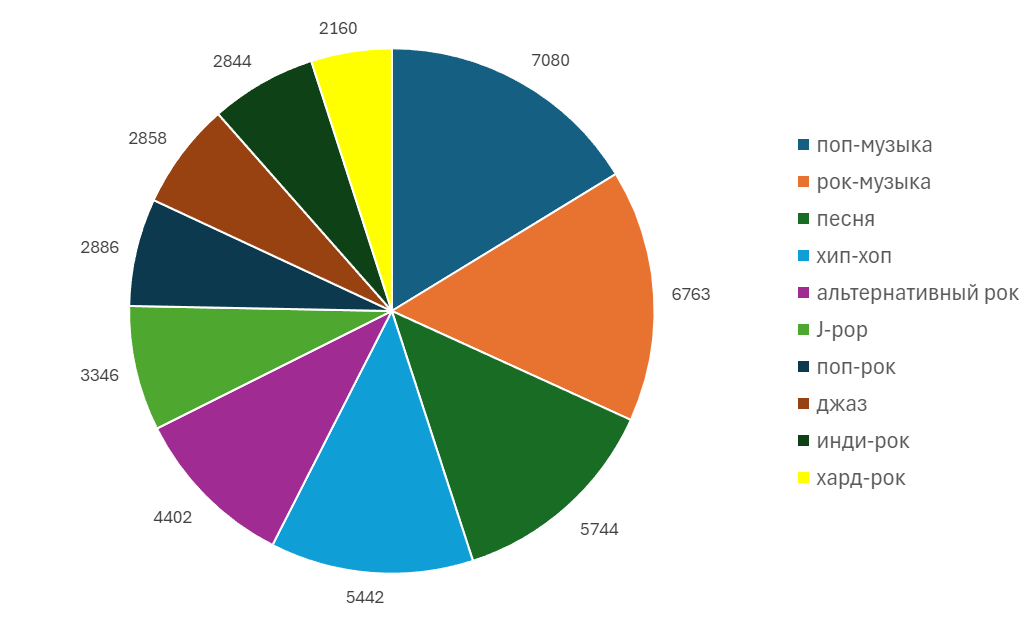
\includegraphics[width=1\textwidth]{./chapter/musical_composition/Genre_Chart_2000-2030.png}
	\caption{Круговая диаграмма числа музыкальных жанров за 2000--2030 годы во всем мире.}%
	\label{fig:Genre_Chart_2000_—_2030}%
\end{marginfigure}

Из результатов запроса~\ref{lst:music_in_genres_1960-1990} 
и~запроса~\ref{lst:music_in_genres_after2020}, можем сделать вывод, 
что жанры музыкальных произведений первого пика, не отличаются от жанров второго. 
На второй диаграмме~\ref{fig:Genre_Chart_2000_—_2030}, видим, что 95,5\,\% музыкальных произведений написаны в жанре <<песня>>. В жанре <<духовная песня>> количество музыкальных произведений по сравнению с рис.~\ref{fig:Genre_Chart_1960_—_1990} уменьшилось почти в 4 раза. А такие музыкальные жанры, как: <<гимн>> и <<музыкальная тема>> на диаграмме~\ref{fig:Genre_Chart_2000_—_2030} по сравнению с диаграммой~\ref{fig:Genre_Chart_1960_—_1990} пропали.

\todoVlad{После предложенных изменений 
запросов~\ref{lst:music_in_genres_1960-1990} 
       и~\ref{lst:music_in_genres_after2020} 
этот абзац с анализом выше нужно будет переработать. И ещё вопросы.\\
1) Если это разные скрипты, то у них это должно быть отражено в названии. Сейчас они совпадают.\\
2) Несправедливое сравнение, поскольку в первом скрипте 1960--1990 (30 лет), 
а во втором только 20 лет (2000--2020). 
Предлагаю увеличить срок во втором скрипте: 2000--2030. 
Почти половина десятилетия уже прошла, это будет более честно сравнивать.}

\todoVlad{Вопросы по~рис.~\ref{fig:Genre_Chart_2000_—_2030}:\\
1) Почему в подписи написано про 10 лет (2000--2010)?\\
2) По запросу~\ref{lst:music_in_genres_after2020} 
не получается построить этот рис.}
\answerVlad{Готово.}



\newpage
\section{Поиск музыкальных лакун в общественном достоянии}

Задача состоит в том, чтобы найти такие музыкальные произведения, 
авторы которых умерли более 70 лет назад, 
и аудиозапись которых отсутствует на Викискладе. 
Найдём и упорядочим такие произведения от самых старых к новым 
с помощью запроса~\ref{lst:music_gaps_in_public_domain}. 
Существует практическая выгода и польза от~такого запроса~\ref{lst:music_gaps_in_public_domain}, 
поскольку видно, какие произведения можно и нужно оцифровывать 
(с~пластинок, кассет) и загружать на~Викисклад для илюстрации статей Википедии.

\begin{lstlisting}[ 
    language=SPARQL,
    caption={\href{https://w.wiki/9f7N}
                  {Отсутствующие аудиозаписи музыкальных произведений, авторы которых умерли 
                   более 70 лет назад }\protect\footnotemark},
    label=lst:music_gaps_in_public_domain,
    texcl,
    numbers=none
    ]
# Search music gaps in public domain
SELECT ?music ?musicLabel ?date
WHERE {
  ?music wdt:P31 wd:Q105543609.	# instance of compostion
  ?music wdt:P86 ?composer.		# composition has a composer
  ?music wdt:P577 ?date.		# composition has a publication date
  ?composer wdt:P570 ?death.			# composer has a date of death
  MINUS {?music wdt:P51 []}.		# compositions without audio 
  FILTER(?death < "1953-01-01T00:00:00Z"^^xsd:dateTime)        # composers that passed away more than 70 years ago
  FILTER(?date < "1953-01-01T00:00:00Z"^^xsd:dateTime)  # compositions that were published more than 70 years ago
  SERVICE wikibase:label { bd:serviceParam wikibase:language "ru,en". }
}
ORDER BY ASC(?date)
\end{lstlisting}%
\footnotetext{Получено: \num{3771} запись на 2017 год, \num{4273} записи на 2023 год и \num{4396} записей на 2024 год. Ссылка на SPARQL-запрос: \href{https://w.wiki/9f7N}{https://w.wiki/9f7N}.}

\todoVlad{Предлагаю во всех скриптах использовать единые переменные,\\ 
то есть ?music, а не ?composition.\\
?date, а не ?publication.}
\answerVlad{Готово.}

В России общественное достояние включает природные ресурсы, культурные объекты, научные достижения и образовательные ресурсы, предназначенные для общего пользования и подлежащие сохранению в соответствии с законодательством. В общем случае произведение переходит в общественное достояние в России, если с года смерти его автора прошло 70 лет. Кроме того, существует <<правило 70+4>>, согласно которому лица, трудившиеся или участвовавшие в Великой Отечественной войне, могут рассчитывать на приоритет в использовании общественных ресурсов.
\footnotetext{URL: \href{https://ru.wikipedia.org/?curid=31363}
                        {https://ru.wikipedia.org/wiki/Общественное\_достояние}.}



\section{Полнота Викиданных}

Проанализируем полноту Викиданных. 
Сравним количесво уникальных композиторов, предоставленных в Викиданных, 
с числом композиторов по другим источникам. 
Также проверим, как изменяется полнота Викиданных со временем, 
сравнив результаты запроса~\ref{lst:BubbleComposers} за~2017 год, 
рис.~\ref{fig:Composers2017} и за~2023 год, рис.~\ref{fig:Composers2023}.

По данным 
\href{https://ru.wikipedia.org/?curid=1362802}
     {<<Музыкального словаря Гроува>>} 
за всю историю человечества существовало \num{20374} композиторов\sidenote{%
                    URL: \href{https://ru.wikipedia.org/?curid=1362802}
                              {https://ru.wikipedia.org/?curid=1362802}.}. 
По данным категории 
\href{https://ru.wikipedia.org/?curid=155531}
     {<<Композиторы по алфавиту>>} 
Русской Википедии существует \num{7800} композиторов\sidenote{%
                    URL: \href{https://ru.wikipedia.org/?curid=155531}
                              {https://ru.wikipedia.org/?curid=155531}.}. 
По данным категории 
\href{https://en.wikipedia.org/?curid=6921880}
     {List of composers by name} 
Английской Википедии существует \num{4958} композиторов\sidenote{%
                    URL: \href{https://en.wikipedia.org/?curid=6921880}
                              {https://en.wikipedia.org/?curid=6921880}.}.
\todoVlad{Нужно обновить данные по словарю Гроува, я по ссылке не нашёл этого числа. 
Или загляните в сам словарь Гроува...\\
Обновите число <<4685 композиторов>> по Английской Википедии~--- нужно подсчитать как-то 
это число по странице, куда ведёт ссылка.} 
\answerVlad{Я не нашел иформации по поводу кличества композиторов по ссылке на словарь Гроува. Но в тексте говорится про онлайн-версию этого словаря, которую до сих пор дополняют. Нашел ссылку на этот словарь и нашел следующую страницу \href{https://www.oxfordmusiconline.com/page/about-gmo/about-grove-music-online}{https://www.oxfordmusiconline.com/page/about-gmo/about-grove-music-online}, на ней гооврится о 33000 биографических статей. Мне добавить это значение с ссылкой на данную страницу? }

Количество музыкальных композиций с заполненным свойством <<\wdProperty{86}{композитор}>> равно \num{3862}, что показывает нам запрос \href{https://w.wiki/56Rc}{https://w.wiki/56Rc}, и это с учётом того, что один композитор мог написать несколько музыкальных произведений. Например, \href{https://ru.wikipedia.org/wiki/Моцарт,_Вольфганг_Амадей}{Вольфганг Амадей Моцарт} написал \num{95} произведений, что существенно снижает количество уникальных композиторов. Полученное число \num{3862}, из результатов запроса \href{https://w.wiki/56Rc}{https://w.wiki/56Rc}, меньше, чем количество композиторов из Русской и Английской Википедии и существенно меньше, чем количество композиторов из \href{https://ru.wikipedia.org/wiki/Музыкальный_словарь_Гроува}{<<Музыкального словаря Гроува>>}, что говорит нам о неполноте Викиданных.

\todoVlad{Скрипты и числа выше устарели. Возможно, скрипты потребуют переделки.}
\answerVlad{Не получается исправить скрипты. Поменял <<\wdqName{музыкальная композиция}{207628}>> на <<\wdqName{музыкальное произведение/композиция}{105543609}>>. Но при выполнении запроса пишет, что запрос занял слишком много времени.}
\begin{marginfigure}[1\baselineskip]
  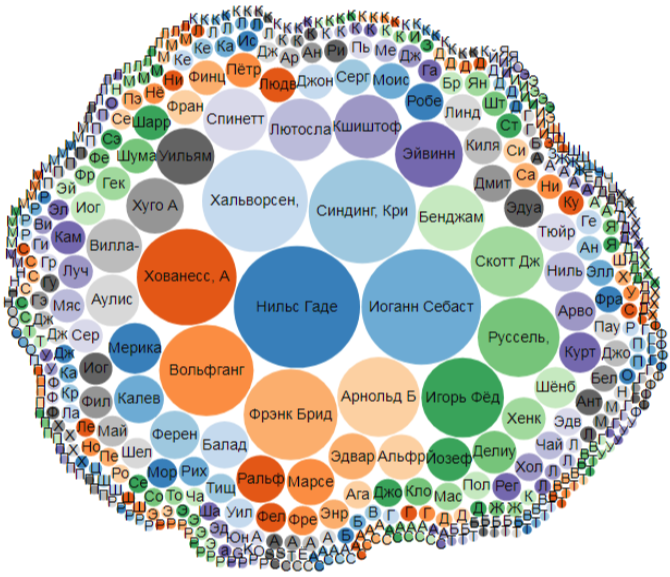
\includegraphics[width=\textwidth]{./chapter/musical_composition/Composer_all_2017.png}
  \vspace{-7pt}
  \caption[Пузырьковая диаграмма композиторов по количеству написанных композиций на~2017 год]{Пузырьковая диаграмма композиторов по количеству написанных композиций на~2017 год}%
  \label{fig:Composers2017}%
\end{marginfigure}

Запрос \href{https://w.wiki/9arZ}{https://w.wiki/9arZ} по композициям с заполненным свойством <<\wdProperty{86}{композитор}>> и свойством <<\wdProperty{495}{страна происхождения}>>, имеющим значения <<\wdqName{Российская империя}{34266}>>, <<\wdqName{СССР}{15180}>> или <<\wdqName{Россия}{159}>>, выдал \num{176} произведений.

\todoVlad{Уже не 8, а 0 произведений. Нет, это говорит не о недостатке данных, 
а о том, что нужно искать по-другому. 
Я думаю, что здесь устарел объект, по которому ищут: composed musical work (Q207628). 
В скриптах в начале главы мы ищем по другим объектам.}
\answerVlad{Готово.}

Запрос~\ref{lst:BubbleComposers} строит пузырьковую диаграмму композиторов по числу написанных ими произведений.
Мы запускали этот скрипт в 2017 году (рис.~\ref{fig:Composers2017}) 
и~в~2023 году (рис.~\ref{fig:Composers2023}).


\begin{lstlisting}[ 
    language=SPARQL, 
    numbers=none,
    caption={\href{https://w.wiki/9are}
                  {Пузырьковая диаграмма композиторов по~числу музыкальных произведений}\protect\footnotemark},
    label=lst:BubbleComposers,
    texcl,
    numbers=none
    ]
# composers with musical compositions
#defaultView:BubbleChart
SELECT ?composer ?composerLabel (COUNT(*) AS ?count) WHERE {
  ?music wdt:P31 wd:Q105543609; # this composition
               wdt:P86 ?composer.     # was written by the composer
  SERVICE wikibase:label { bd:serviceParam wikibase:language "ru, en" }
}
GROUP BY ?composer ?composerLabel
ORDER BY DESC(?count) ?composerLabel
\end{lstlisting}%
\footnotetext{Получено: \num{773} записи. Ссылка на SPARQL-запрос: \href{https://w.wiki/9are}{https://w.wiki/9are}.}

Размер круга означает количество написанных музыкальных композиций. Диаграмма показывает, что у одних композиторов значительно больше композиций чем у других. В~первую пятерку входят \href{https://ru.wikipedia.org/wiki/Гаде,_Нильс}{Нильс Гаде} (\num{173} композиции), \href{https://ru.wikipedia.org/wiki/Бах,_Иоганн_Себастьян}{Иоганн Себастьян Бах} (\num{155} композиций), \href{https://ru.wikipedia.org/wiki/Синдинг,_Кристиан_Август}{Кристиан Август Синдинг} (\num{125} композиций), \href{https://ru.wikipedia.org/wiki/Хальворсен,_Юхан}{Юхан Хальворсен} (\num{121} композиция), \href{https://ru.wikipedia.org/wiki/Хованесс,_Алан}{Алан Хованесс} (\num{108} композиций).

%
%
\begin{marginfigure}
  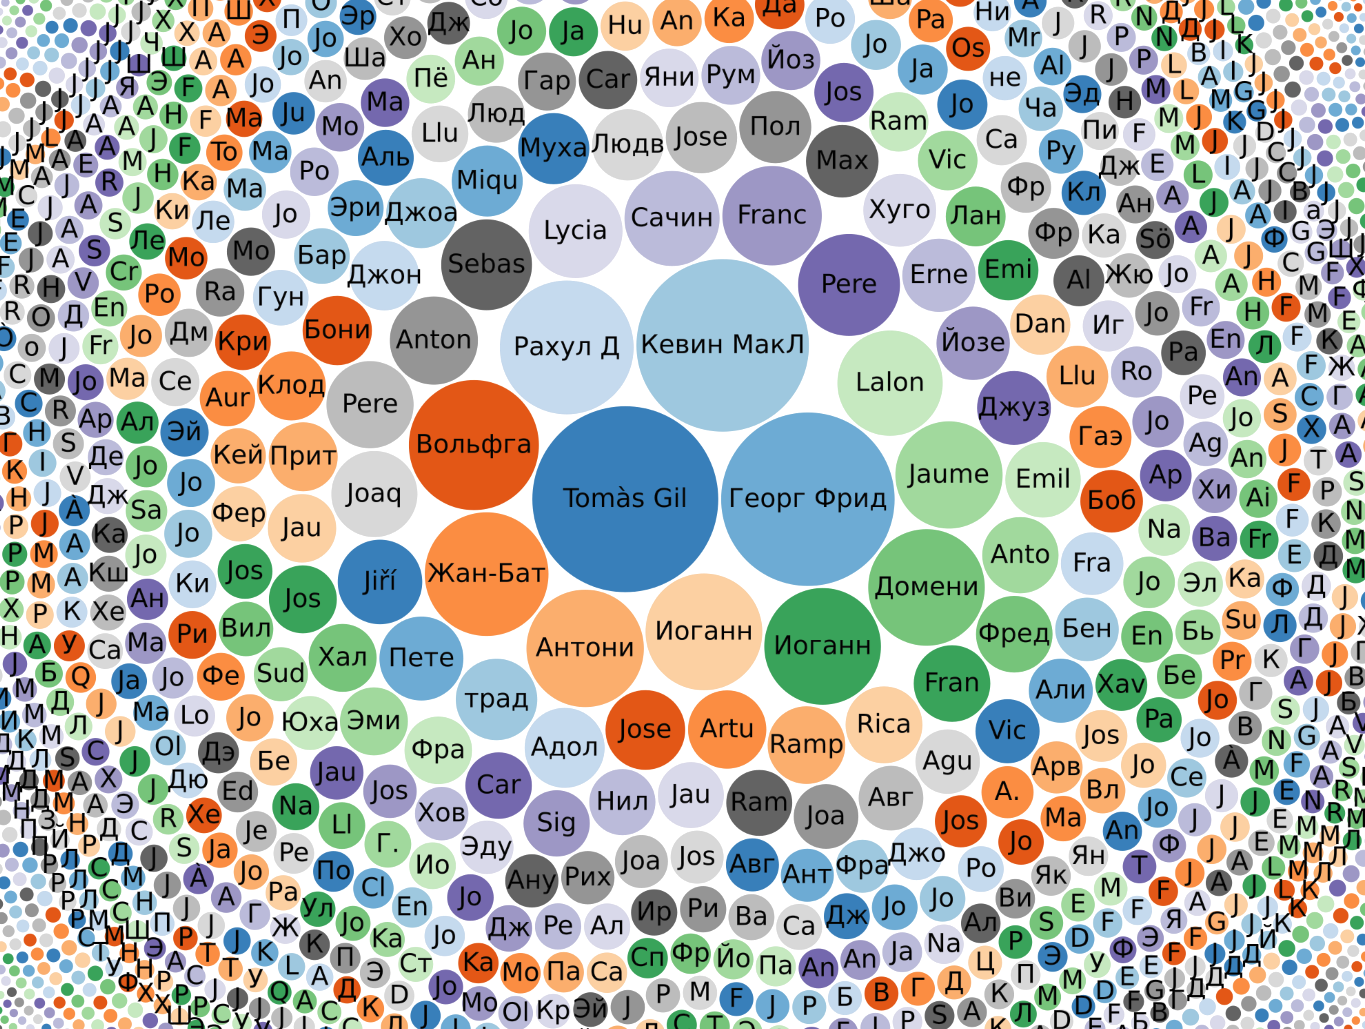
\includegraphics[width=\textwidth]{./chapter/musical_composition/Composer_all_2023_box.png}
  \vspace{-7pt}
  \caption[Пузырьковая диаграмма композиторов по количеству написанных композиций на~2023 год]
    {Фрагмент диаграммы композиторов по количеству написанных произведений на~2023 год}%
  \label{fig:Composers2023}%
\end{marginfigure}

Диаграмма~\ref{fig:Composers2023} за 2023 год позывает, 
как изменилось количество написанных композиций у различный композиторов. 
Чтобы рассмотреть подробнее, 
добавим в конец запроса~\ref{lst:BubbleComposers} строку  \lstinline|LIMIT 12|, 
чтобы ограничить количество записей до 12, 
получим следующий запрос \href{https://w.wiki/8A2h}{https://w.wiki/8A2h}, 
результат на рис.~\ref{fig:12composers}. 

\todoVlad{По рис.~\ref{fig:12composers}. 
С помощью запроса Вы получаете SVG-файл. Внутри этого файла найдите текст с именами 
композиторов в кружках. Увеличьте в несколько раз размер шрифта. 
Если не влезает в строку, то добавьте перенос строки в ФИО. 
Потом перегоняйте в PNG. Сейчас имена на рис. нечитабельны. 
}

Сравним результаты за~2017 год и за~2023 год.
По сравнению с 2017 годом в первую пятёрку входят 
\href{https://ca.wikipedia.org/wiki/Tomàs_Gil_i_Membrado}{Томас Хиль Мембрадо} 
(\num{1437} композиций), 
\href{https://ru.wikipedia.org/wiki/Гендель,_Георг_Фридрих}{Гендель Георг Фридрих} (\num{1251} композиция), 
\href{https://ru.wikipedia.org/wiki/Маклауд,_Кевин}{Маклауд Кевин} (\num{1237} композиций), 
\href{https://en.wikipedia.org/wiki/R._D._Burman}{Рахул Дев Бурман} (\num{744} композиции), 
\href{https://ru.wikipedia.org/wiki/Моцарт,_Вольфганг_Амадей}{Вольфганг Амадей Моцарт} (\num{703} композиции). 
Исходя из данных диаграмм~\ref{fig:Composers2017} и ~\ref{fig:Composers2023}, 
можно сделать вывод, что появились новые композиторы, 
которые имеют значительно больше композиций. 
При этом у такого классика, как 
\href{https://ru.wikipedia.org/?curid=17950}{Иоганн Себастьян Бах}, 
число композиций увеличилось за эти годы на 411 и составило 566. 

\newpage
\begin{marginfigure}
  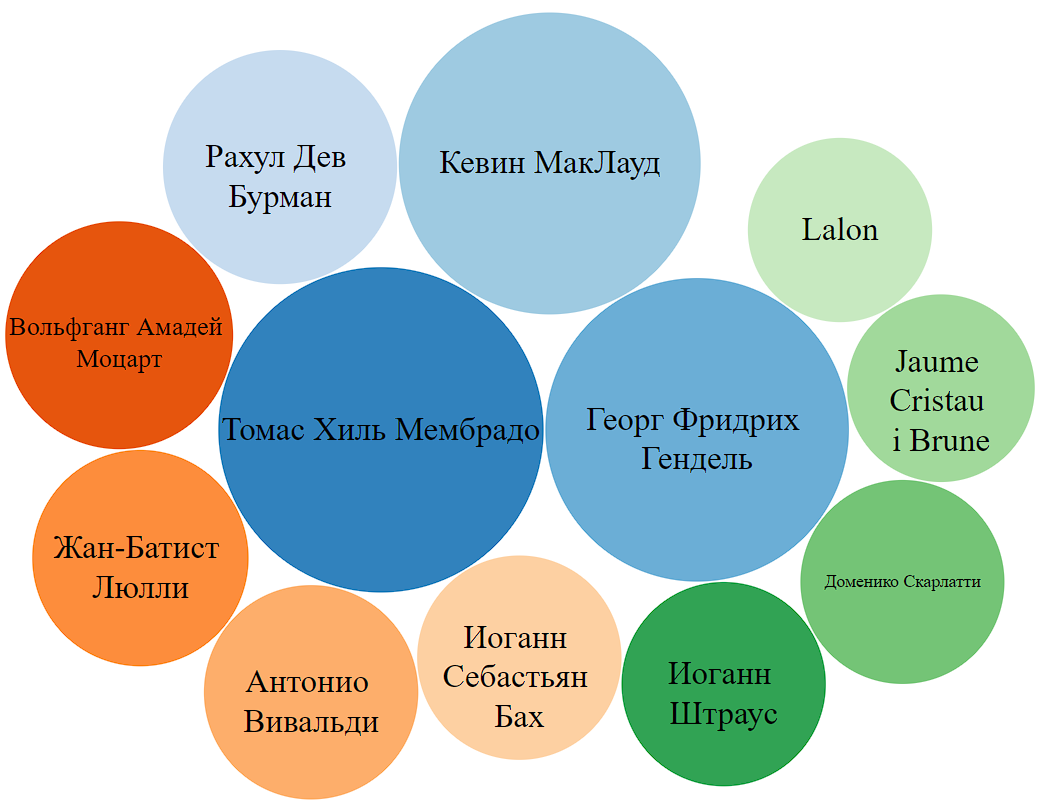
\includegraphics[width=\textwidth]{./chapter/musical_composition/Composers_12_at_2023.png}
  \caption[Диаграмма 12 композиторов с наибольшим количеством написанных музыкальных композиций на~2023 год]
          {Пузырьковая диаграмма 12 композиторов с наибольшим количеством написанных музыкальных композиций на~2023 год}%
  \label{fig:12composers}%
\end{marginfigure}


\section{Упражнения}
\begin{enumerate}
\item Найти список музыкальных композиций, созданных во время эпохи классицизма (XVII--XVIII века).
Используйте свойство <<\wdProperty{571}{дата создания}>>.
\item Найти композитора, который написал больше симфоний, чем остальные. 
    Используйте свойства <<\wdProperty{31}{экземпляр}>>, <<\wdProperty{86}{композитор}>>
        и объект <<\wdqName {симфония} {9734}>>.
\item Построить гистограмму, на которой отображается количество музыкальных композиций 
        группы The Beatles по году публикации.
        Используйте свойства: <<\wdProperty{175}{исполнитель}>>, <<\wdProperty{577}{дата публикации}>>.

        \label{question:TheBeatles_quest}
        См. ответ~\ref{lst:TheBeatles} на с.~\pageref{answer:TheBeatles_answ}.


\todoVlad{Запрос ниже вместе с пояснениями перенесите в раздел Ответы 
        и свяжите взаимными ссылками вопрос и ответ.\\
        В названии запроса и в подписи к рисунку укажите 
        временные рамки, по которым идёт запрос. 
        В тексте поясните, почему именно эти годы 
        (кстати, это хорошо видно, если снять ограничение по годам). 
} 
\answerVlad{Готово.}
\end{enumerate}
